\section{Circuit Fabrication and Assembly}\label{sec:printed-circuit-board}

	\subsection{PCB Design}\label{ssec:pcb-design}

		The PCB layout for this project was developed using the Altium Designer 17 Software \cite{AD17}. During the layout design some things were considered to ensure functionallity:

		\begin{itemize}
			\item Instead of soldering the connectors directly to the board, empty pads for soldering wires were placed, this way connectors can be chosen later and fixed on the board housing instead of on the board surface.\label{itm:pcb-pin-bars}
			\item Protection devices such as TVS, Fuses and current limiting resistors were placed very close from the terminal pads in order to prevent cooper tracks to be damaged.\label{itm:pcb-protection}
			\item SMT (Surface Mount Technology) was a priority during design in order to save space on the board.\label{itm:pcb-smt}
			\item Cooper tracks width: The width of every track was choosen according to the electrical signal it is carrying.\label{itm:pcb-track}
 		\end{itemize}

 		Figures \ref{fig:pcb-design-top} and \ref{fig:pcb-design-bottom} shows respectively the top and the bottom side of the board during design, most of empty spaces were replaced by ground planes in order to make the board corrosion faster and to make a stronger gnd connection. Other interesting fact is the width of power supply tracks, it is easy to notice they are much more thick than normal signal tracks. The board dimmensions are 130mm x 80mm.

		\begin{figure}[htbp]
			\centering
			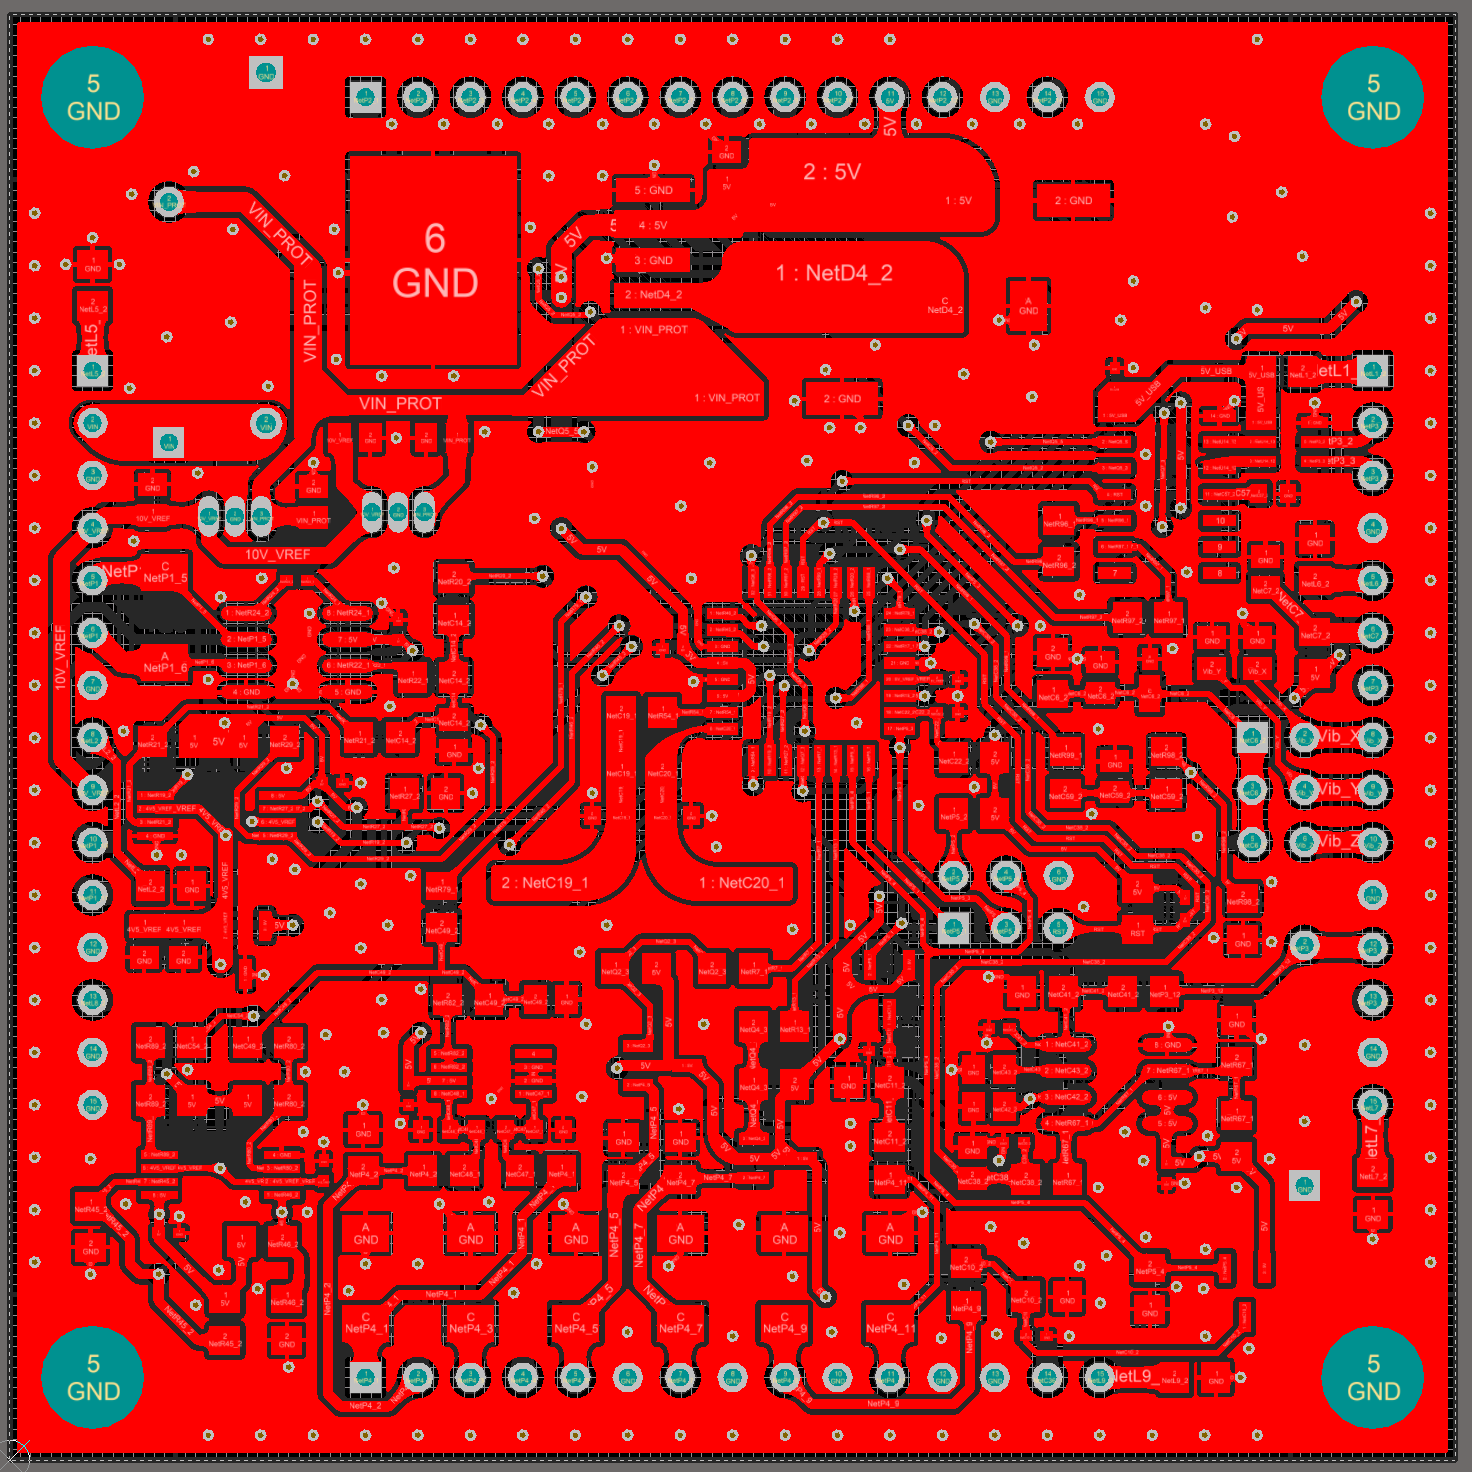
\includegraphics[width=.8\textwidth]{figuras/fig-pcb-design-top}
			\caption{PCB Top 2D View}
			\label{fig:pcb-design-top}
		\end{figure}

		\begin{figure}[htbp]
			\centering
			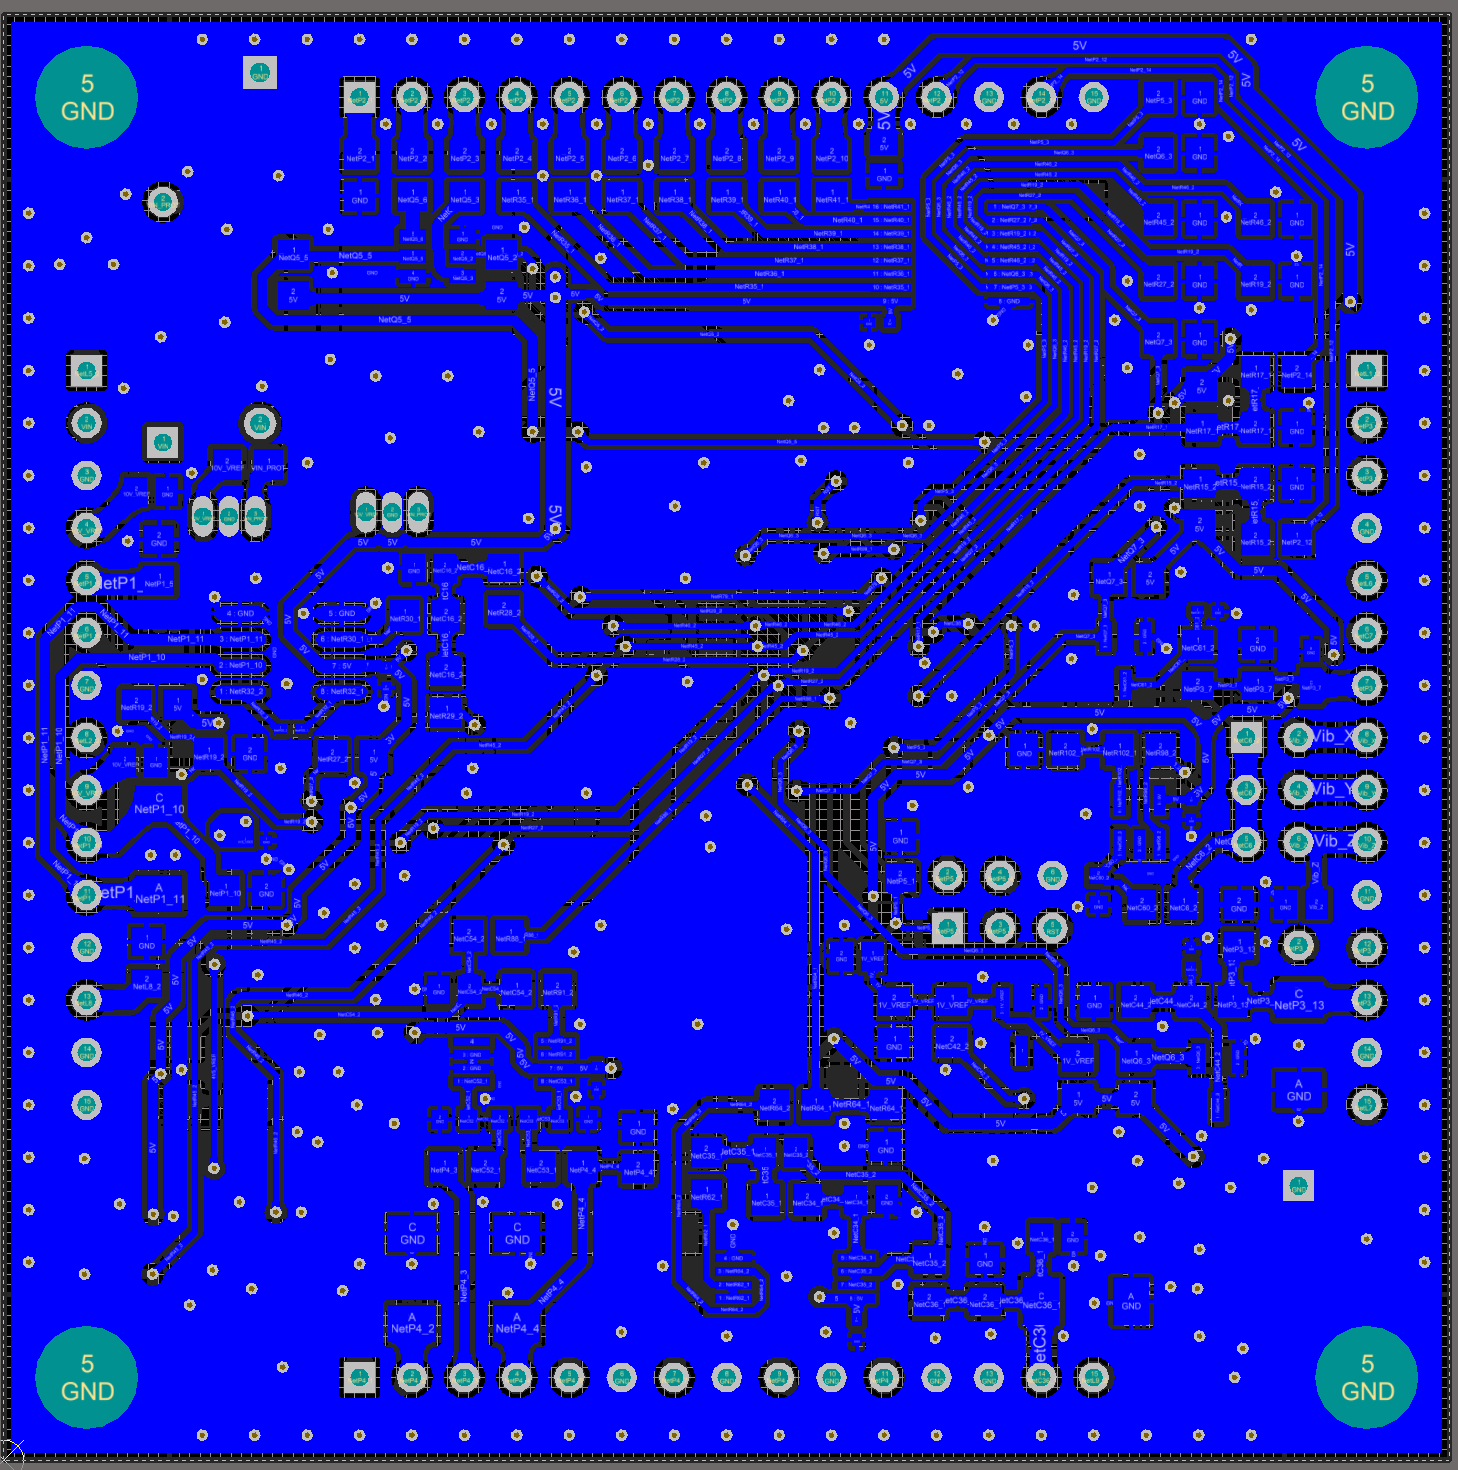
\includegraphics[width=.8\textwidth]{figuras/fig-pcb-design-bottom}
			\caption{PCB Bottom 2D View}
			\label{fig:pcb-design-bottom}
		\end{figure}

		\begin{figure}[htbp]
			\centering
			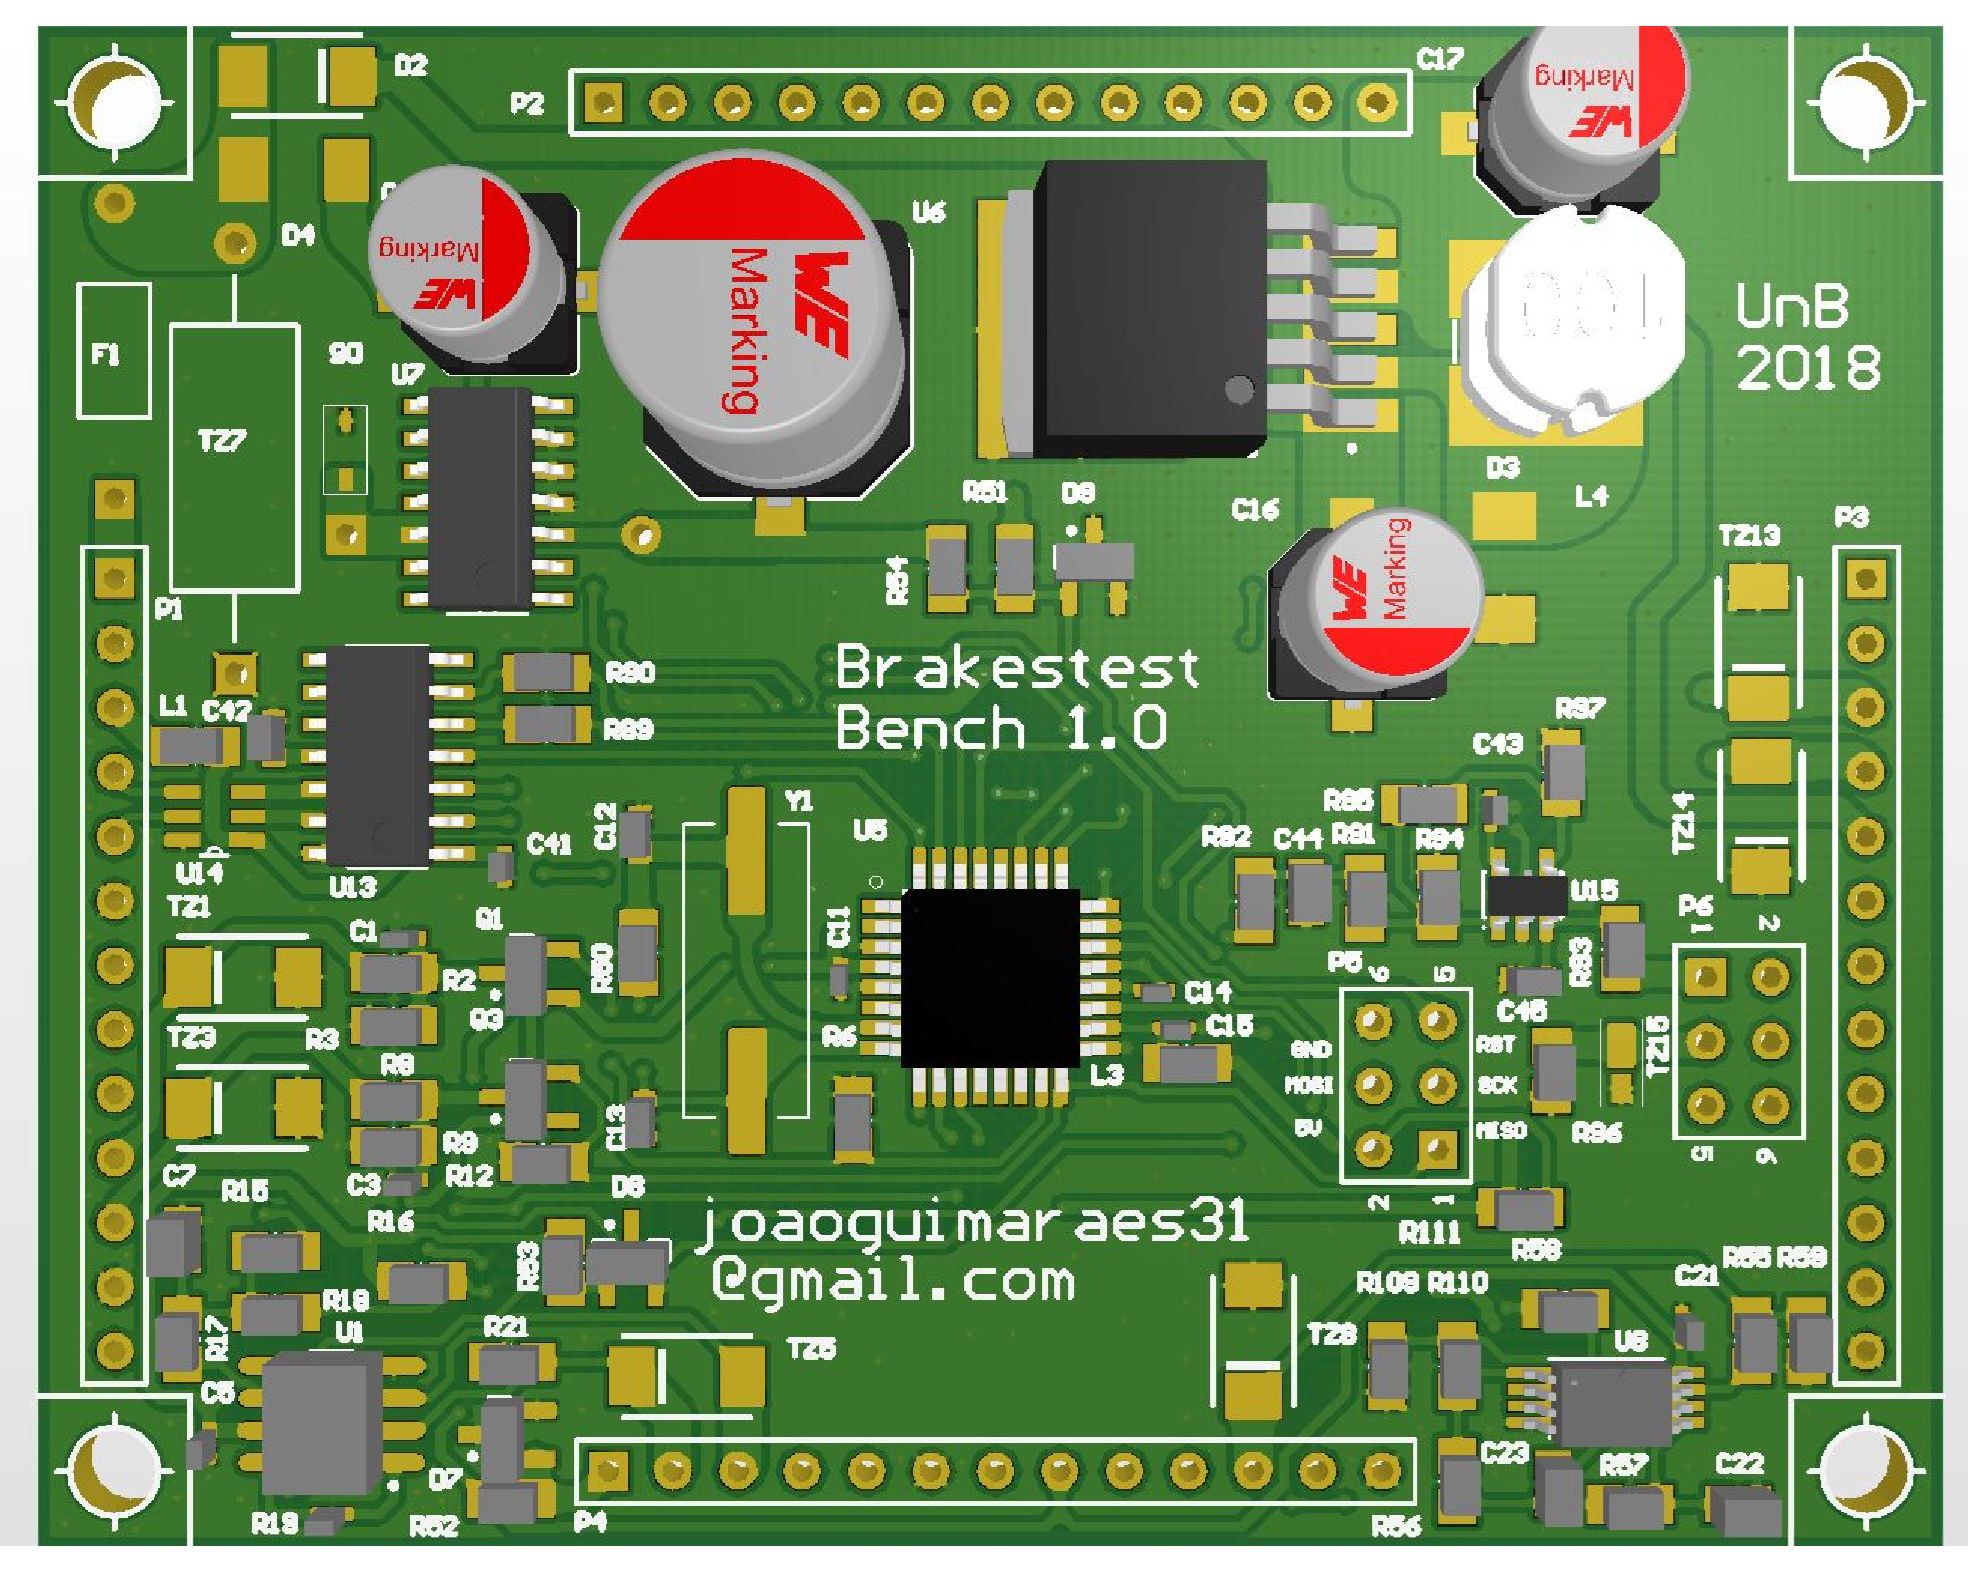
\includegraphics[width=.8\textwidth]{figuras/fig-pcb-print-top}
			\caption{PCB Top View}
			\label{fig:pcb-print-top}
		\end{figure}

		\begin{figure}[htbp]
			\centering
			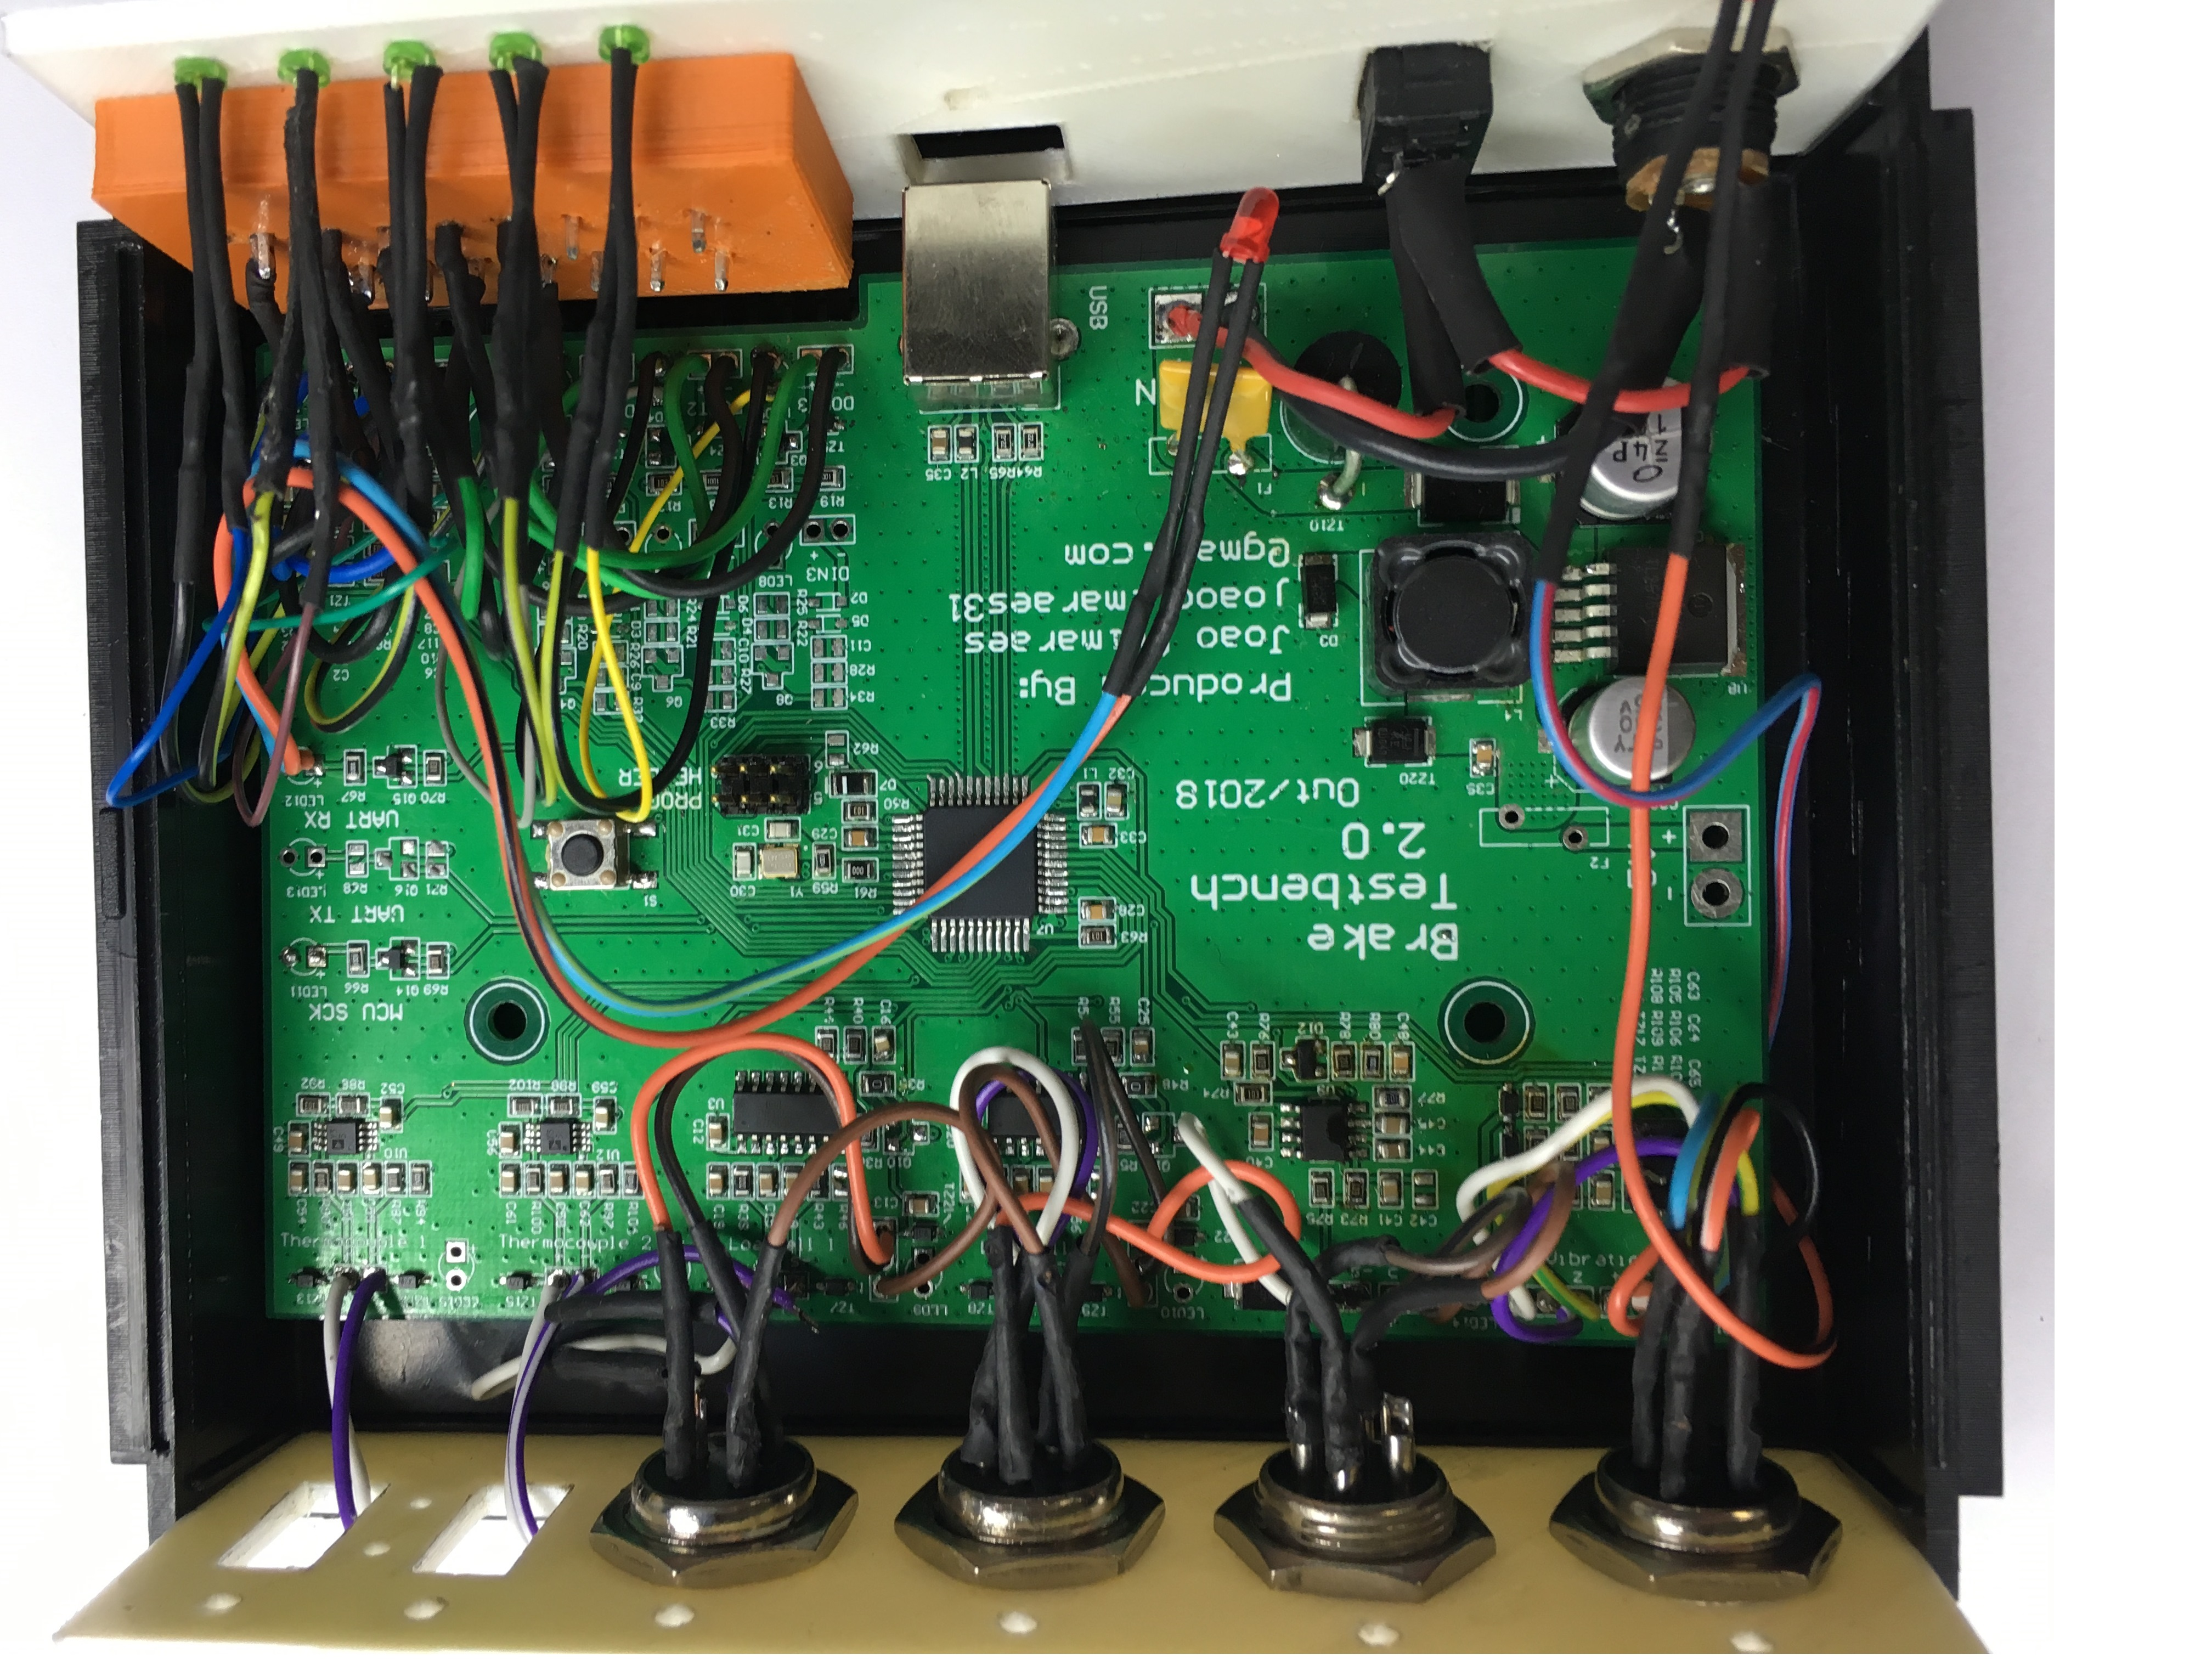
\includegraphics[width=.8\textwidth]{figuras/fig-pcb-real}
			\caption{Real PCB Assembled}
			\label{fig-pcb-real}
		\end{figure}